% nie rusza�
\RequirePackage{ifpdf}
\newif\ifelektroniczna
\newif\ifjednostronna
\newif\ifprojektInzynierski

%%%%%%%%%%%%%%%%%%%%%%%%%%%%%%%%%%%%%%%%%%%%%%%%%%%%%%%%%%%%%%%%%%%%%%%%%%%%
% USTAWIENIA GLOBALNE I domy�lna �cie�ka do plik�w z obrazkami, kodowanie itp. 
% okre�lone s� w drugiej sekcji ustawie�

% czy projekt czy praca magisterska
\projektInzynierskitrue % projekt
%\projektInzynierskifalse % praca magisterska

% czy wersja elektroniczna (pdf z kolorowymi linkami) czy nie (np. do druku)
\elektronicznatrue
%\elektronicznafalse

% czy jednostronna (recenzent), czy dwustronna (do akt);
% UWAGA: to nie jest dyrektywa dla drukarki; nie zmienia sposobu wydruku, 
% tylko to, w jaki spos�b rozpoczynane s� rozdzia�y, ustawiane marginesy
% itp.

%\jednostronnafalse
\jednostronnatrue

%%%%%%%%%%%%%%%%%%%%%%%%%%%%%%%%%%%%%%%%%%%%%%%%%%%%%%%%%%%%%%%%%%%%%%%%%%%%


% nie rusza�
\ifjednostronna
    \def\strony{oneside,openany}
\else
    \def\strony{twoside,openright}
\fi

\ifpdf
    % uwaga, ustawiaj�c co� innego ni� 12 sprawd� uk�ad strony tytu�owej (marginesy)
    \documentclass[pdftex,12pt,a4paper,\strony,colorlinks,nocenter,noupper,crosshair]{thesis}
    \usepackage[pdftex]{graphicx}
    \pdfcompresslevel=1
\else    
    \documentclass[12pt,a4paper,\strony,nocenter,noupper,crosshair]{thesis}
    \usepackage{graphicx}
\fi

% nie rusza�
\usepackage{url}
\usepackage{stronatytulowa}

%%%%%%%%%%%%%%%%%%%%%%%%%%%%%%%%%%%%%%%%%%%%%%%%%%%%%%%%%%%%%%%%%%%%%%%%%%%%
% USTAWIENIA GLOBALNE - cz�� 2
%

% kodowanie dokumentu
%\usepackage[utf8]{inputenc}   % linuks/windows/mac; pozwala na �atwe mieszanie znak�w z r�nych j�zyk�w
\usepackage[cp1250]{inputenc} % windows

% dane 
\ifprojektInzynierski
    \def\rodzaj{Projekt z Biometrii}
\else
    \def\rodzaj{Praca dyplomowa magisterska}
\fi
%\def\rodzaj{Praca przej�ciowa}

% stan na 2011-2012
\ifprojektInzynierski
    \def\wydzial{In�ynierii Biomedycznej}
\else
    \def\wydzial{In�ynierii Biomedycznej}
\fi

\def\tytul{Czytnik lini papilarnych} % Prosz� u�y� i ma�ych, i du�ych liter!
\def\autor{Autor: Dawid Bara�ski, Dawid Nyderek, Kamil Kozie�} %Jan Kowalski a NIE JAN KOWALSKI

% tytu� i autor dla pdfa - najcz�ciej jw, ale bez podzia�u na liniie i BEZ POLSKICH LITER
\def\tytulpdf{dawid_baranski_sprawozdanie}
\def\autorpdf{Dawid Baranski}

% promotor
\def\promotor{Prowadz�cy: dr in�. Marta Danch-Wierzchowska} % prof. nzw. dr hab. in�. dr n.med doc. Jan Kowalski

% z konsultantem/bez konsultanta
%\def\konsultant{Konsultant: Konsultant} prof. nzw. dr hab. in�. dr n.med doc. Jan Nowak
\def\konsultant{}

\def\data{Zabrze, czerwiec, 2019} % uwaga na wielko�� liter: grudzie� 2012/czerwiec 2012/..

% do pdfa
\def\slowakluczowe{SLOWA,KLUCZOWE}

% �cie�ka do obrazk�w
\graphicspath{{./rysunki/}}

% ustawienia dla pdfa
\ifpdf
\ifelektroniczna
     \usepackage[pdfusetitle=true,
	  pdfsubject={\tytulpdf},
	        pdfkeywords={\slowakluczowe}, 
		pdfcreator={\autorpdf},
		pdfstartview=FitV,
		linkcolor=blue,
		citecolor=red,
		]{hyperref}
\fi                 
\fi


\usepackage{layout}% poka� marginesy

% Nazwa za��cznik�w 
\def\appendixname{Za��cznik}
%%%%%%%%%%%%%%%%%%%%%%%%%%%%%%%%%%%%%%%%%%%%%%%%%%%%%%%%%%%%%%%%%%%%%%%%%%%%

% nie rusza� (cho� chwilowo niepotrzebne)
%	\author{\autor}
%	\title{\tytul}
%	\date{\data}
%

% === PAKIETY ===
\usepackage{url}

% �adne czcionki dla PDF + ustawienia spolszczaj�ce
\usepackage{t1enc,amsmath}
\usepackage[OT4,plmath]{polski}

% potrzebne dla strony tytu�owej:
\usepackage{helvet} 

% pierwszy paragraf w rozdziale/sekcji powinien by� wci�ty
\usepackage{indentfirst}

% marginesy
%\usepackage{anysize}
%\marginsize{3cm}{2.5cm}{2.5cm}{2.5cm}%LPGD
%\setlength{\textheight}{24cm}
% za spraw� thesis
%\textwidth 150mm
%\textheight 225mm

% czcionki matematyczne
\usepackage{amsfonts}

% rysunki z�o�one z wielu [pod]rysunk�w
\usepackage{subfig}
\captionsetup[subfigure]{justification=centerfirst}

% mo�liwo�� sklejania wierszy tabeli
\usepackage{multirow}

% mo�liwo�� wklejania adres�w - jest ju� w��czony wy�ej
%\usepackage{url}

% ulepszona obs�uga cytowa�
\usepackage{cite}

% listingi
\usepackage{listings}
% domy�lne ustawienia (niestety utf8 nie jest akceptowany)
%\lstset{language={Matlab},inputencoding=cp1250}}
%\lstset{language={Matlab},inputencoding=latin2}}
\lstset{language={Java},inputencoding=latin2} % powinno pasowa� te� do C#

% \addcontentsline nie dzia�a za dobrze w po��czeniu z hyperref, ale to nie dzia�a z klas� thesis
%\usepackage[nottoc]{tocbibind}

% strona po cleardoublepage powinna by� pusta, nie z nag��wkami
\usepackage{cleardpempty}

% == opcjonalne

% wymu� po�o�enie grafiki (itp.) przez [H]
\usepackage{float} 

% znak promila i inne znaki specjalne
%\usepackage{textcomp}

% je�li trzeba obr�ci� stron� (wstawi� co� w orientacji poziomej), u�yj tych pakiet�w
%\ifpdf\usepackage{pdflscape}\else\usepackage{lscape}\fi

% je�li potrzebujesz d�ugich tabeli (wiele stron)
%\usepackage{longtable}

% === POLECENIA DODATKOWE ===

% wektor w tek�cie
\def\vec#1{\ensuremath{\mathbf{#1}}}

% anglicyzmy i �acinizmy
\def\ang#1{ang.~\emph{#1}}
\def\lat#1{�ac.~\emph{#1}}

% proste e (jako podstawa logarytmu naturalnego) we wzorach i w tek�cie:
\def\e{\ensuremath{\textrm{\normalfont{}e}}}

% znak stopnia [jak w "5 stopni"]
\def\stopien{\ensuremath{^{\circ}}\protect\space}

% notatki na marginesie
\def\fixme#1{\marginpar{\tiny{}#1}}
%\def\fixme#1{} % gdy nie chcemy ich drukowa�, wystarczy zast�pi� powy�sze tym

%ODNOSNIKI 
% �eby wykorzysta� przypis dwukrotnie; druga wersja gorzej dzia�a�a w po��czeniu 
% z hyperref; czyli \footnote{blablabla \label{przypisX}} + \footnotereuse{przypisX}
%\newcommand{\footnreuse}[1]{\raisebox{1ex}{\scriptsize{}\protect\ref{#1}}}

% == �RODOWISKA DLA TWIERDZE�, LEMAT�W itp. ===
\newtheorem{twierdzenie}{Twierdzenie}[chapter]
\newtheorem{wlasnosc}{W�asno��}[chapter]
\newtheorem{lemat}{Lemat}[chapter]
\newenvironment{dowod}{\parindent=0pt{\bf Dow�d. }}{\begin{flushright}$\square$\end{flushright}}

% === RACZEJ NIE RUSZA� ===

%\usepackage{makeidx}
%\makeindex
%\usepackage{threeparttable}
%\usepackage[small,center]{caption2}

\def\captionlabeldelim{.}

%\usepackage{geometry}
%GATHER{thesis.bib}
%\usepackage[twoside]{geometry}
%\geometry{ lmargin=3.5cm, rmargin=2.5cm, tmargin=3cm, bmargin=3cm,
%headheight=1cm, headsep=0.5cm, footskip=0pt }

\linespread{1}
\chapterfont{\Huge\bfseries}
\sectionfont{\bfseries\Large}
\subsectionfont{\bfseries\large}
\institutionfont{\bfseries}%\mdseries}
\def\captionlabelfont{\bfseries}

\renewcommand{\figureshortname}{Rys.}
\renewcommand{\tableshortname}{Tab.}

\renewcommand\floatpagefraction{.9}
\renewcommand\topfraction{.9}
\renewcommand\bottomfraction{.9}
\renewcommand\textfraction{.1}
\setcounter{totalnumber}{50}
\setcounter{topnumber}{50}
\setcounter{bottomnumber}{50}

\newcommand{\topcaption}{%                  % robi podpis nad tabelk� z odst�pem po podpisie
   \setlength{\abovecaptionskip}{0pt}%
   \setlength{\belowcaptionskip}{10pt}%
   \caption}



% marginesy
\usepackage{anysize}
\marginsize{3cm}{2.5cm}{2.5cm}{2.5cm}%LPGD
%\setlength{\textheight}{24cm}
% za spraw� thesis
%\textwidth 150mm
%\textheight 225mm

\begin{document}
%
\bibliographystyle{acm}
%

%
\stronatytulowa
\titlepage
%-\cleardoublepage % je�li dwustronnie, to druga strona powinna by� pusta
\frontmatter 
%\maketitle

%\tocbibname

\tableofcontents \listoffigures \listoftables
%\listofacros
%\input{abbrev_body}
%\newpage
%\input{spis_oznaczen}

\mainmatter % <--- to + frontmatter powy�ej odpowiada za fakt, �e numerowanie jest od 1!
\renewcommand{\arraystretch}{1.2}

\chapter{Wst�p}
\section{Cel projektu}
Celem pracy by�a analiza biometrycznych system�w zabezpiecze� opartych na odczycie linii papilarnych w urz�dzeniach u�ytku codziennego oraz implemetacja autoryzacji dost�pu 
do aplikacji mobilnej przy pomocy czytnika linii papilarnych. 
\section{Zakres pracy}
Zakres pracy:
\begin{enumerate}
\item Analiza wykorzystywanych system�w biometrycznych.
\item Analiza dost�pnych czytnik�w linii papilarnych.
\item Analiza metod implementacji czytnik�w linii papilarnych w aplikacjach.
\item Implementacja obs�ugi autoryzacji dost�pu do aplikacji poprzez czytnik linii papilarnych:

\begin{enumerate}
\item przygotowanie widok�w,
\item opracowanie API,
\item po��czenie widok�w i API z istniej�c� aplikacj�.
\end{enumerate}

\item Opracowanie podsumowania i wniosk�w.
\end{enumerate}


\section{Wst�p teoretyczny}
\subsection{Systemy biometryczne}
Biometria jest nauk� zajmuj�c� si� pomiarami i analiz� cech fizycznych i behawioralnych organizm�w �ywych. Dane te wykorzystywane s� w wielu innych dziedzinach nauki kryminologii, antropologii, fizjologii, medycynie[1, 2].
Najcz�ciej spotykanym zastosowaniem metod biometrycznych jest kontrola dost�pu 
w systemach zabezpiecze�. Systemy takie mog� za pomoc� danych biometrycznych udziela� dost�pu do systemu b�d� okre�lonych danych jedynie osobom do tego uprawnionym. Mocn� stron� tego rozwi�zania jest indywidualno�� cech, kt�re s� wykorzystywane.
Cechami biometrycznymi nazywamy indywidualne atrybuty, kt�re charakteryzuj� si� znikom� powtarzalno�ci� w obr�bie populacji. Do cech takich zaliczamy mi�dzy innymi:
\begin{itemize}
\item odcisk palca,
\item wz�r t�cz�wki oka,
\item g�os,
\item zapach,
\item ch�d,
\item podpis.
\end{itemize}

Najbradziej rozpowszechnion� cech� wykorzystywan� do autoryzacji dost�pu jest analiza linii papilarnych. Czytniki linii papilarnych motowane s� w wi�kszo�ci wsp�czesnych smartphon�w, mog� zas�powa� klucz do drzwi lub by� alternatywnym sposobem logowania si� do komputera.
Cechy biometryczne mierzone kilkukrotnie u tego samego cz�owieka, charakteryzuj� 
si� zmienno�ci� dla poszczeg�lnych pomiar�w. Wi��e si� to z zale�no�ci� tych cech od stanu psychofizycznego cz�owieka, warunk�w otoczenia czy interakcji u�ytkownika z czujnikiem[3]. Wynikiem tego jest brak mo�liwo�ci okre�lenia stuprocentowej zgodno�ci wzorca z innym  pomiarem danej cechy.

\subsection{Czytniki linii papilarnych}
\begin{figure}[!htb]
	\centering
	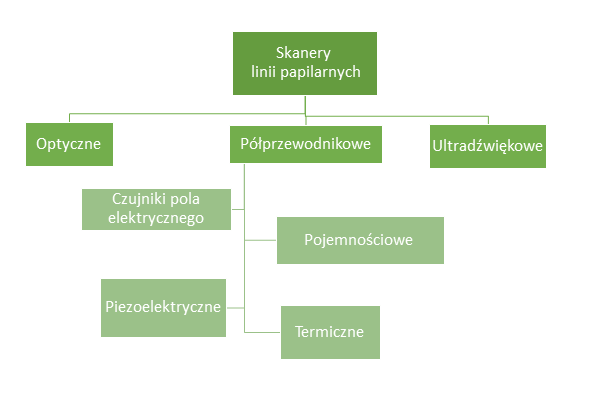
\includegraphics[width=.8\textwidth]{skanery}
	\caption{Skanery linii papilarnych.}\label{l:skanery}
\end{figure}
Praktyka wykorzytywania cech biometrycznych do identyfikacji, weryfikacji oraz autoryzacji os�b za pomoc� cech biometrycznych wi��e si� z behawioralnym przystosowaniem cz�owieka. Ma to miejsce za ka�dym razem kiedy rozpoznajemy ludzi na podstawie twarzy. Umiej�tno�� ta wykorzystywana jest przez ludzi cz�sto nie �wiadomie.
�wiadome wykorzytywanie cech biometrycznych mia�o jednak miejsce ju� 500 p.n.e. kiedy to zacz�to wykorzystywa� odcisk palca do rejestracji transakcji. W po�niejszym okresie, 
za spraw� M. Malpighi�ego oraz J. C. A. Mayer�a, odcisk palca a w�a�ciwie jego cechy zosta�y opisane oraz stwierdzono ich unikatowo��. Dzi�ki pracy tych os�b na ko�cu XIX w. stworzony zosta� pierwszy kompletny system klasyfikacji os�b na podstawie odcisk�w palca. Autorem prac by� Sir E. Henry [4]. Pomiar�w dokonywano na odbitych na papierze palc�w wcze�niej zamoczonych w tuszu.
Dzi� do pomiar�w odcisk�w palc�w wykorzystuje si� czytniki odcisk�w palc�w. Skanery linii papilarnych, ze wzgl�du na ykorzystywan� metod� pomiaru mo�emy podzieli� 
na optyczne, p�przewodnikowe oraz ultrad�wi�kowe. Skanery optyczne b�d�ce, jednymi
z pierwszych stosowanych, wykorzystuj� zjawisko odbicia �wiat�a. Najcz�ciej obraz zbierany jest z serii jednowymiarowych zestaw�w danych, kt�rych wychwycenie nast�puje na skutek przeci�gni�cia palcem po czujniku. Tworzony przez takie czujniki dwuwymiarowy obraz jest z�o�eniem tych kawa�k�w, przy wykorzystaniu algoryt�w rekonstrukcyjnych [5]. Podzia� skaner�w zosta� przedstawiony na rysunku (Rys.~\ref{l:skanery}).

\begin{figure}[!htb]
	\centering
	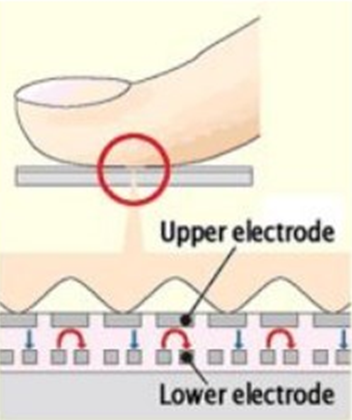
\includegraphics[width=.6\textwidth]{czujnik}
	\caption{Schemat dzia�ania czujnika pojemno�ciowego.}\label{l:czujnik}
\end{figure}

W przypadku budowy macierzowej, kt�re jednocze�nie pozwala zebra� ca�o�� obrazu, rejestracja sygna�u odbywa si� przy wykorzystaniu kamer CMOS.
Wykorzystanie zjawiska odbicia �wiat�a pozwala, na stosunkowo proste, podrobienie odcisku palca. Metoda ta, w wersji podstawowej, nie pozwala wkry� cz�owiecze�stwa badanego obiektu. Nowocze�niejsze, dro�sze wersje czytnik�w pozwalaj� okre�li� cz�owiecze�stwo 
dzi�ki, na przyk�ad pomiaowi natlenowania krwi w naczyniach wie�cowych.
Najnowszymi pod wzgl�dem wykorzystania technologi s� czytniki ultrad�wi�kowe. Wykorzystuj� one to samo falowe zjawisko co czujniki optyczne. Ich przewag� jest mo�liwo�� ukrycia ich pod os�onami. Wykorzystywane jest to w telefonach kom�rkowych, w kt�rych czytniki takie umieszczane s� pod ekranem. Dzi�ki temu s� nie widoczne dla oczu, daj�c mo�liwo�� autoryzacji u�ytkownikowi.
Najcz�ciej stosowanymi z czujnik�w s� czujniki p�przewodnikowe. Ich budowa najcz�ciej sprowadza si� do dwuwarstwowej macierzy p�przewodnik�w tworz�cymi pewien rodzaj kondensatora. Mierzona jest pojemno�� tych kondensator�w, kt�ra zmienia si� je�eli 
do wierzchniej strony przy�o�ony zostanie palec. Do zmiany pojemno�ci konieczny jest �ywy palec, lub kopia z odpowiedniego materia�u, jest on zatem bezpieczniejszy od czujnika optycznego [5,6]. Schemat dzia�ania czujnika linii papilarnych zosta� przedstawiony na rysunku (Rys.~\ref{l:czujnik}).

\chapter{Projekt}
\section{Rozwi�zanie problemu}
\subsection{Wykorzystane technologie}
\begin{table}[]
\centering
\caption{Szczeg�y wykorzystanych technologii.}
\label{l:technologie}
\begin{tabular}{|l|l|}
\hline
\textbf{Zakres}            & \textbf{Wykorzystana technologia}                \\ \hline
System operacyjny          & Android (wersja \textgreater = 7.1)              \\ \hline
�rodowisko programistyczne & Android Studio                                   \\ \hline
J�zyk programowania        & Java                                             \\ \hline
Baza danych                & SQLite                                           \\ \hline
Technologia autoryzacji    & Android Fingerprint API, Bibliteki: Volley, Gson \\ \hline
\end{tabular}
\end{table}

Do stworzenia implementacji modu�u autoryzacji dost�pu do aplikacji wykorzystano r�ne technologie. Zosta�y one wymienione w tabeli (Tab.~\ref{l:technologie}).

\subsection{Widoki modu�u}
\begin{figure}[!htb]
	\centering
	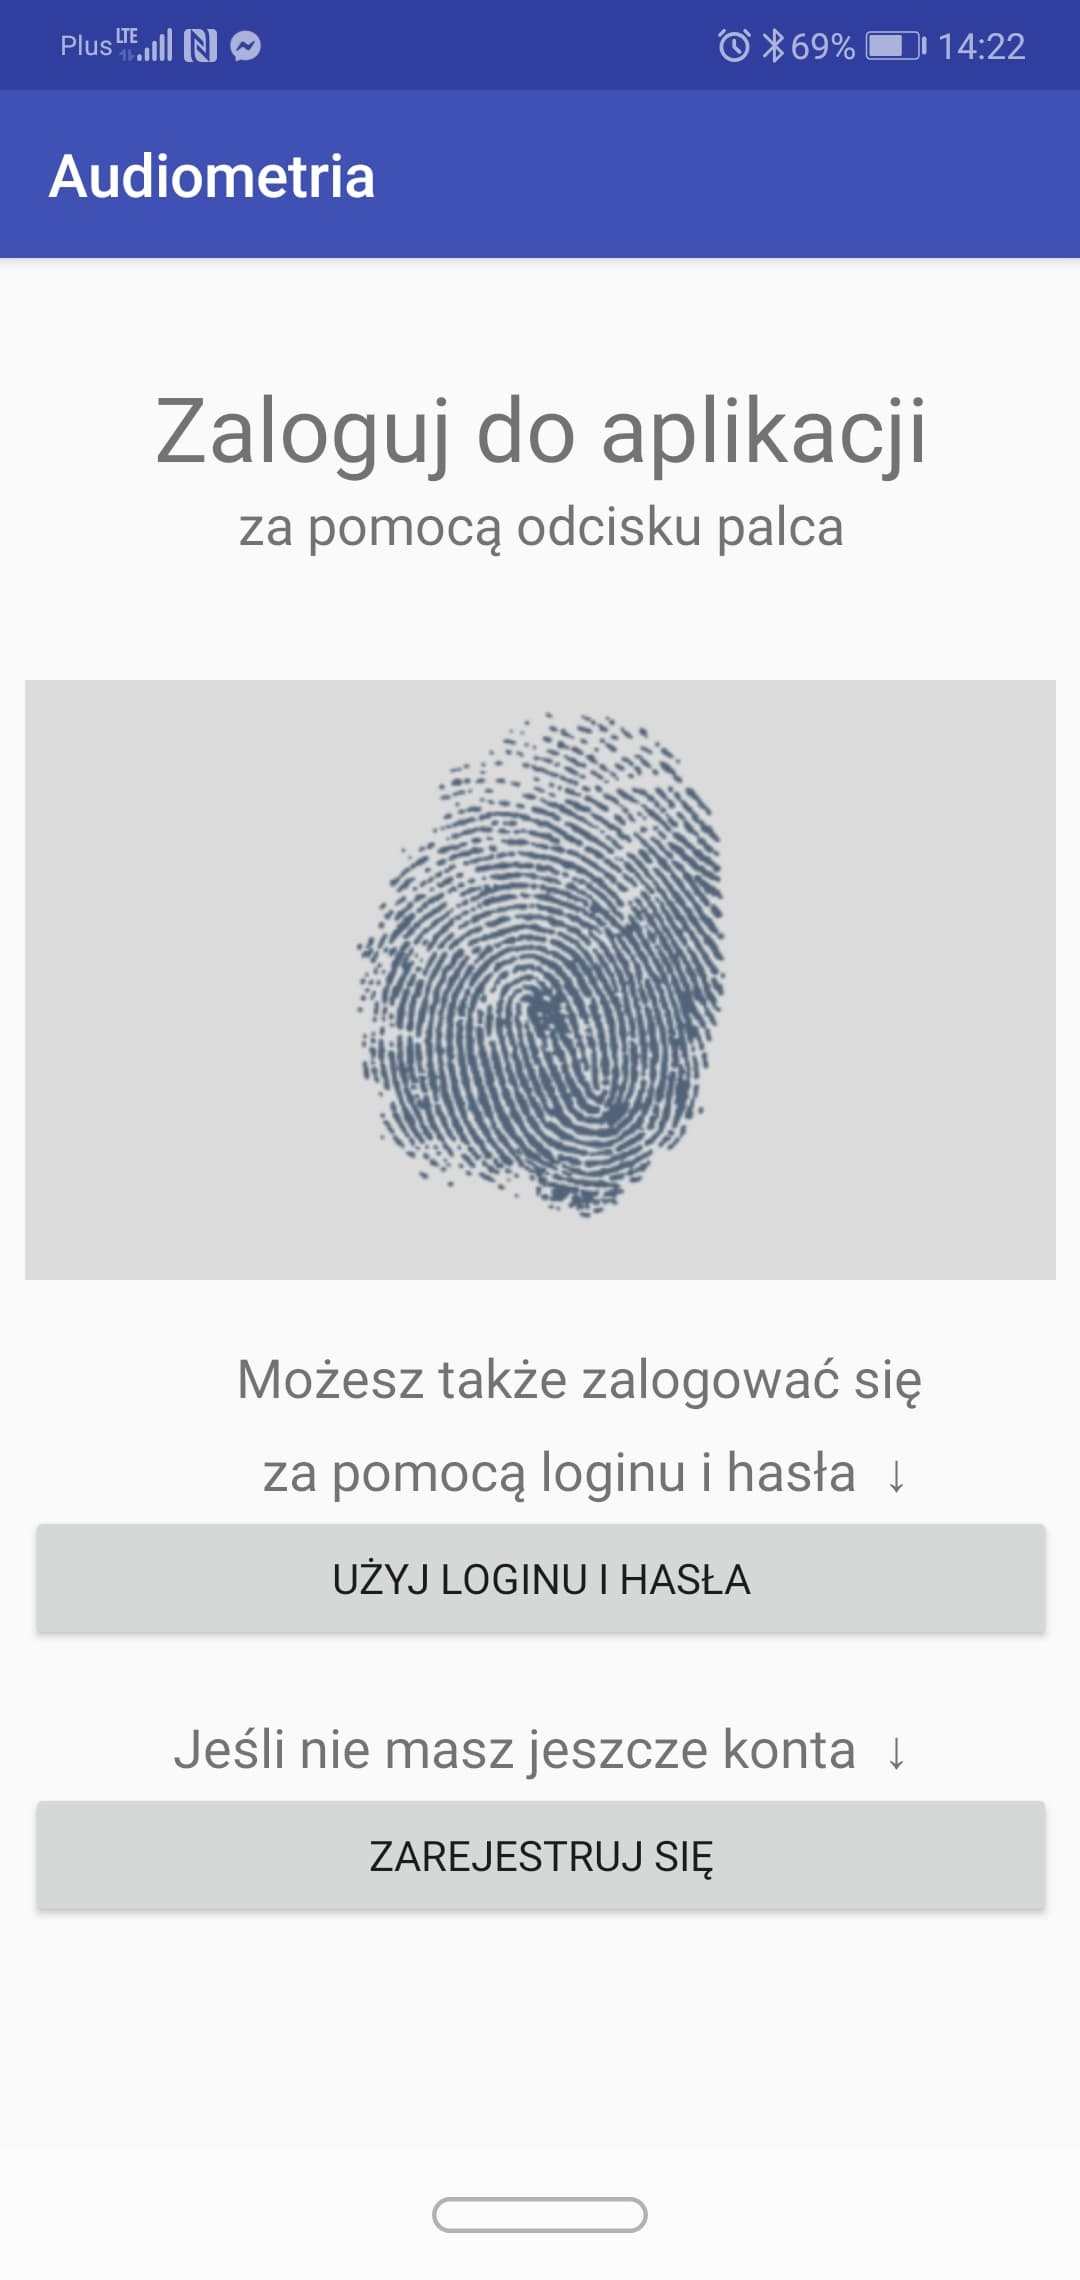
\includegraphics[width=.5\textwidth]{widok2}
	\caption{Powitalny widok logowania odciskiem palca.}\label{l:widok2}
\end{figure}	

\begin{figure}[!htb]
	\centering
	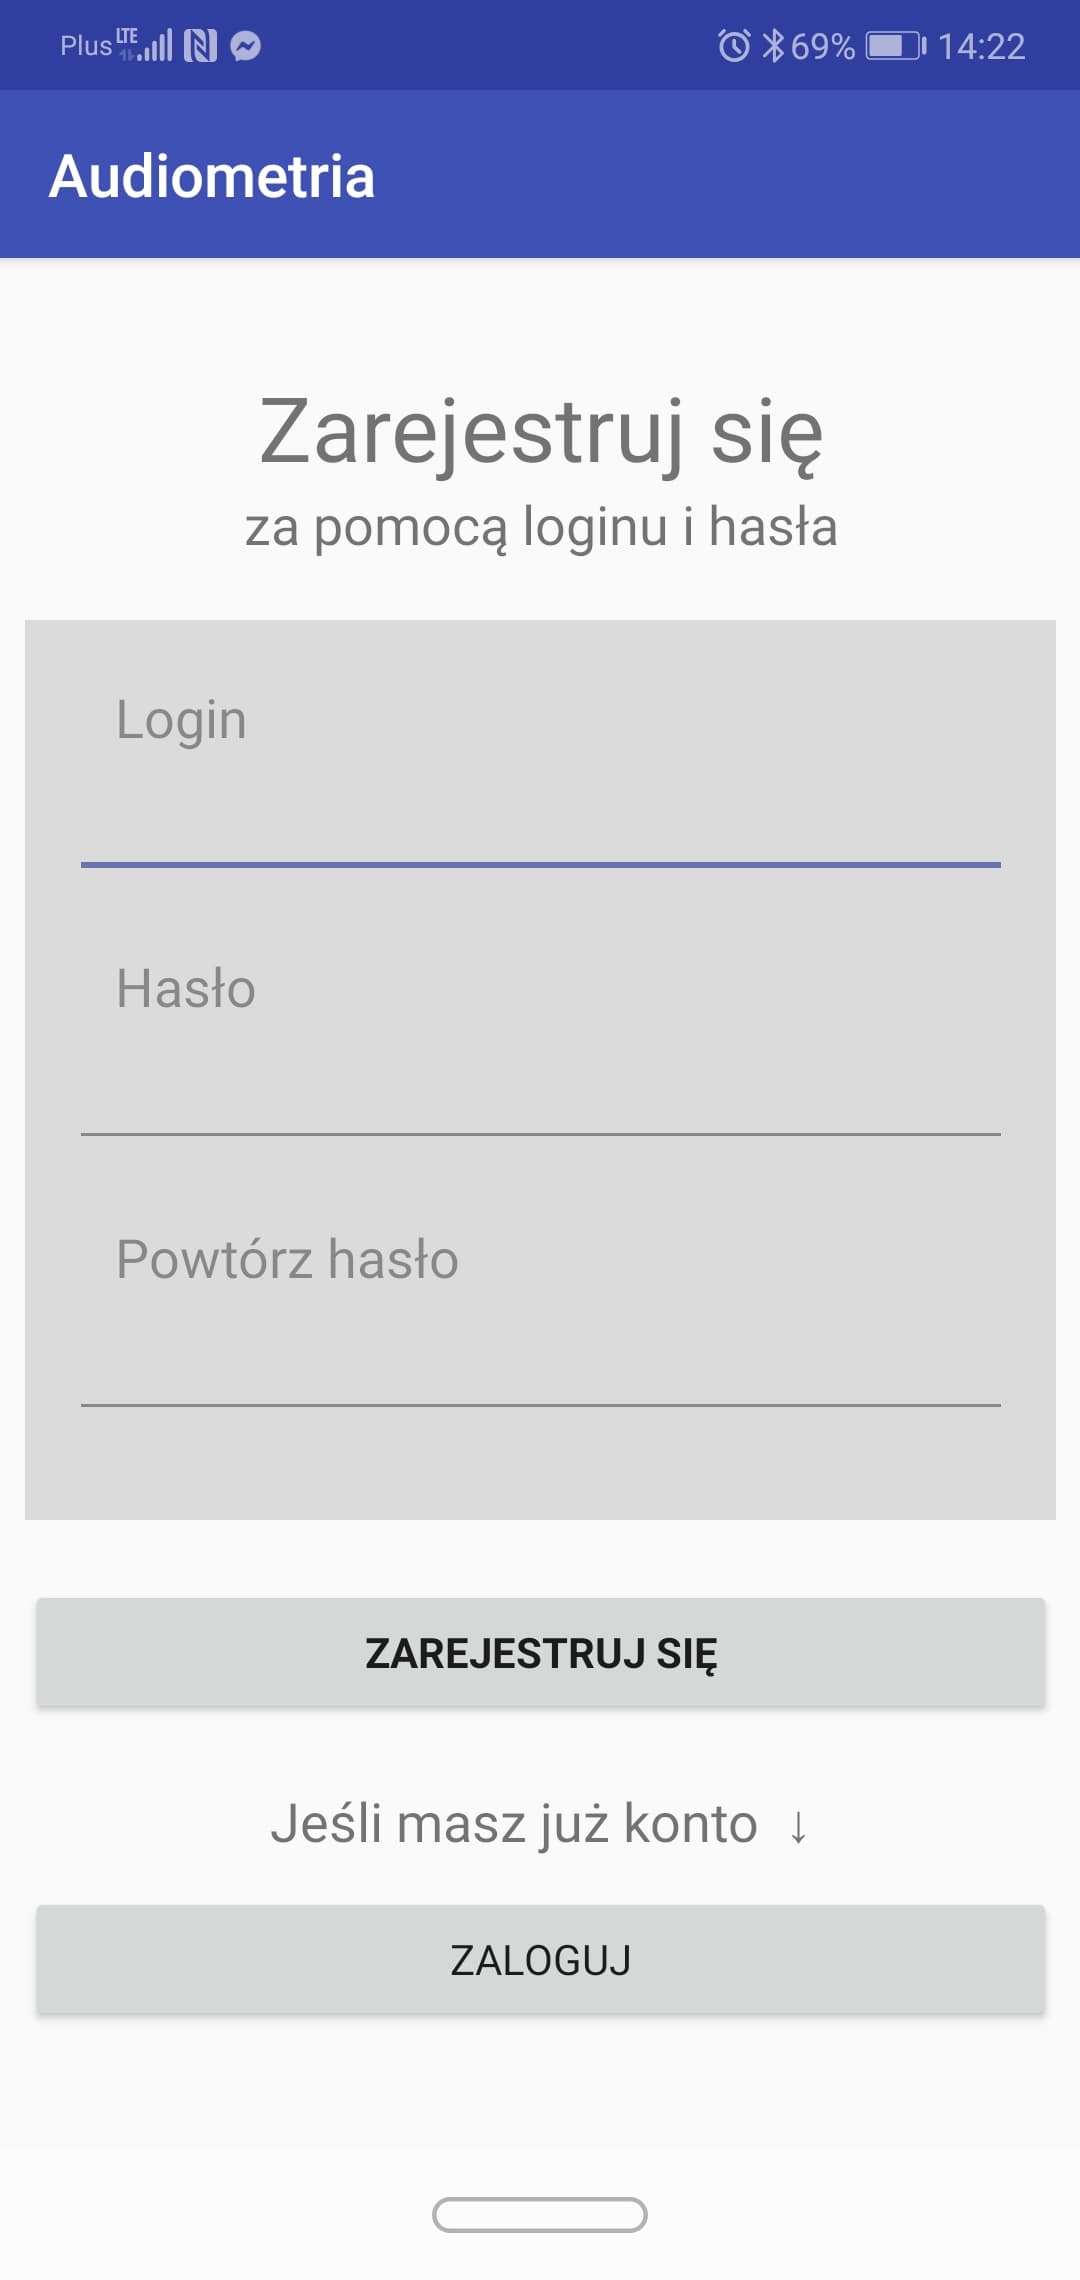
\includegraphics[width=.5\textwidth]{widok1}
	\caption{Widok rejestracji.}\label{l:widok1}
\end{figure}

\begin{figure}[!htb]
	\centering
	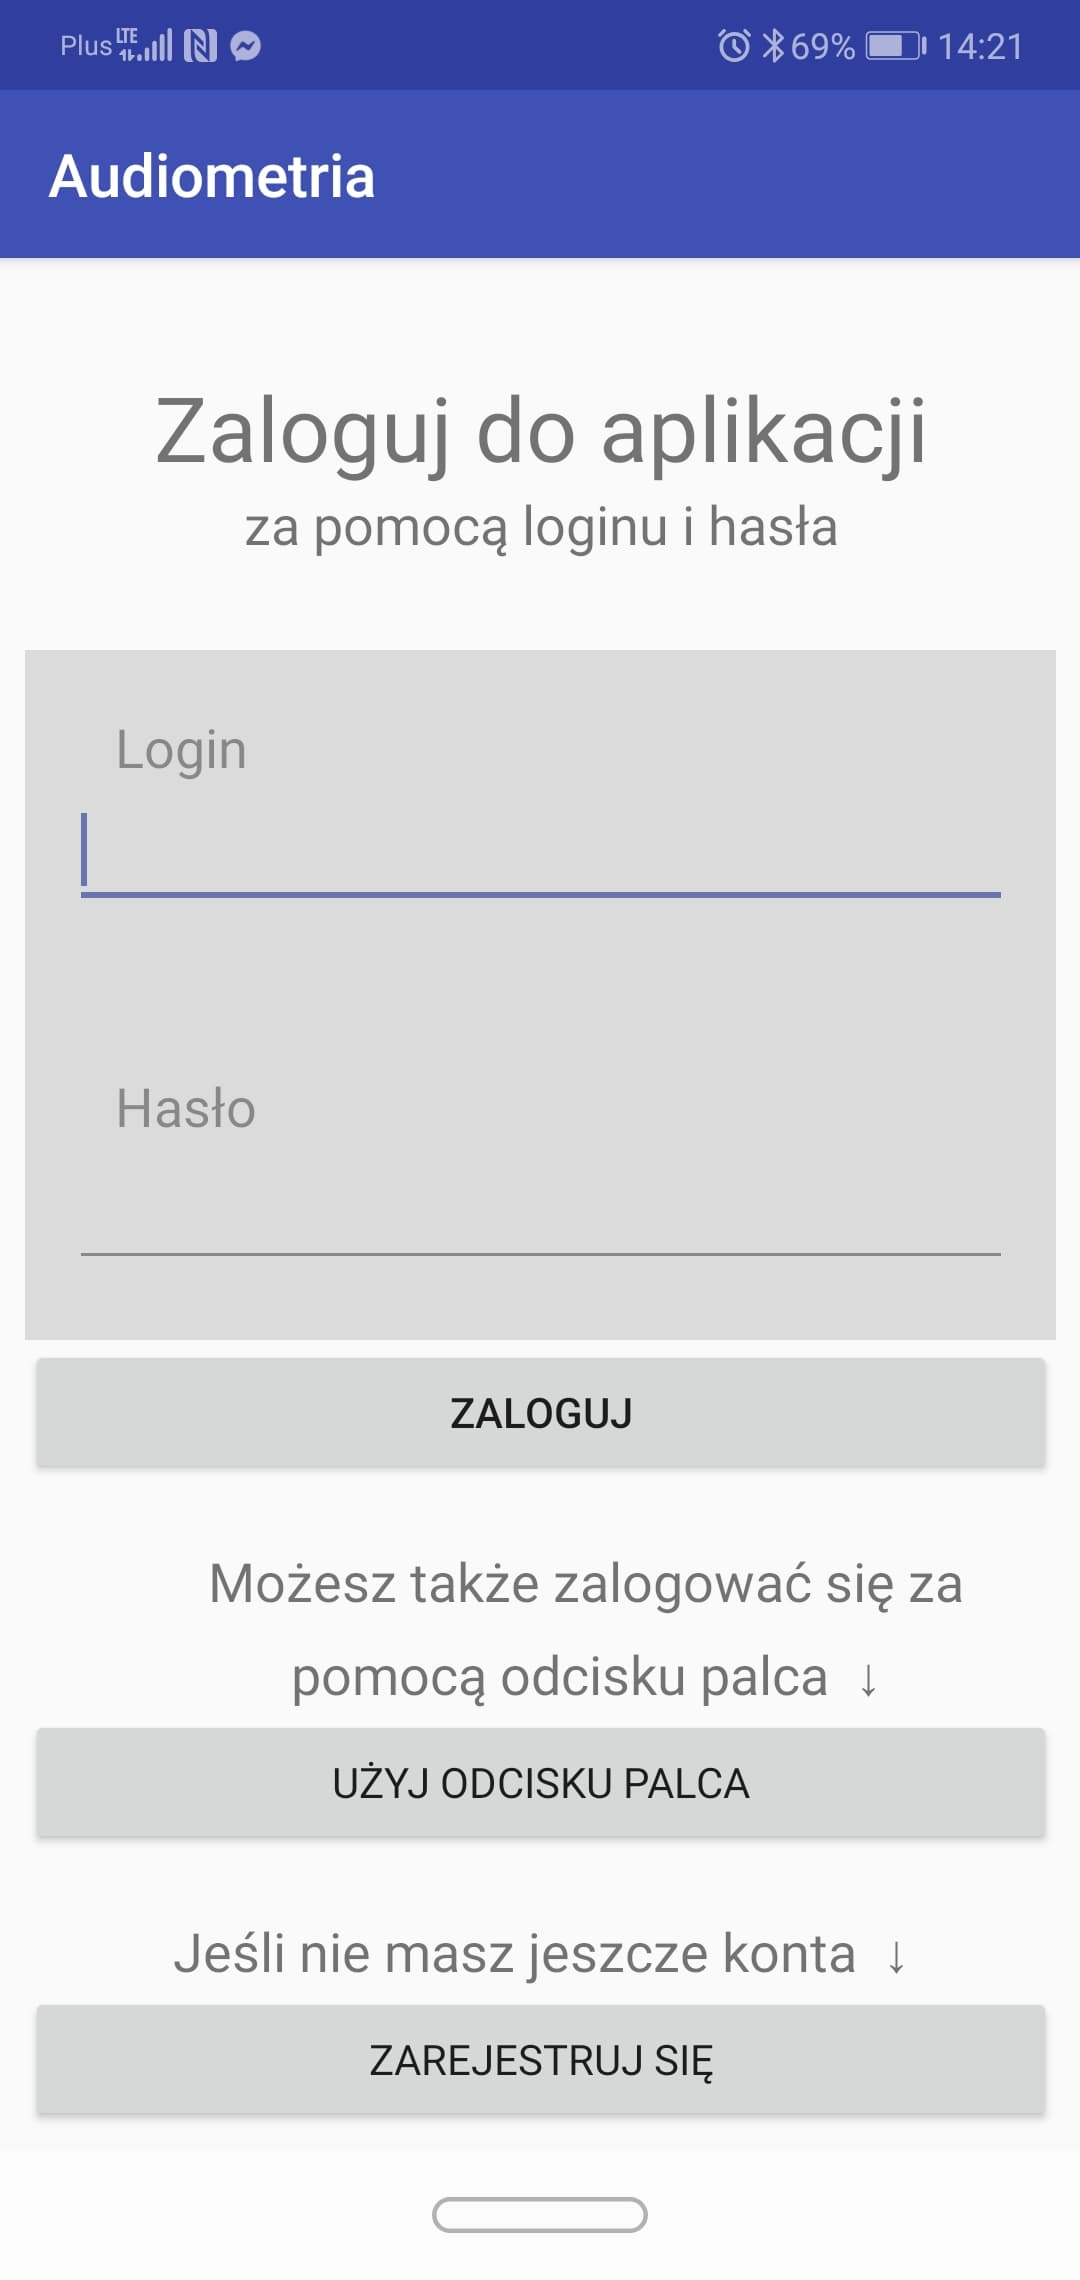
\includegraphics[width=.5\textwidth]{widok3}
	\caption{Widok tradycyjnego logowania.}\label{l:widok3}
\end{figure}

Przygotowany modu� obs�ugiwany jest przy pomocy trzech widocznych na rysunkach widok�w (Rys.~\ref{l:widok1}, \ref{l:widok2}, \ref{l:widok3}). Widoki zaprojektowane zosta�y w Adobe XD, a nast�pnie przygotowane w programie Android Studio.

\subsection{Utworzone API}
\subsection{Po��czenie aplikacji}
\subsection{U�ytkowanie}
Przygotowany modu� pozwala na logowanie si� do zasob�w aplikacji za pomoc� dw�ch metod. Pierwsz� z metod jest wykorzystanie do tego celu loginu i has�a. Drug� metod� jest wykorzystanie odcisku palca, kt�ry jest zarejestrowany w specjalnie przeznaczonej do tego cz�ci pami�ci telefonu. O ile logowanie wy��cznie przy pomocy pierwszej metody mo�e funkcjonowa� samodzielnie, jednak autoryzacja biometryczna wymaga dodatkowego niezale�nego rodzaju logowania. Wi��e si� to z r�nicami cech biometrycznych tej samej osoby w zale�no�ci na przyk�ad od otaczaj�cego �rodowiska.
Ponadto modu� posiada formularz umo�liwiaj�cy rejestracj� nowego u�ytkownika, wymagaj�c� okre�lenia tylko danych do pierwszego rodzaju autoryzacji.
Poszczeg�lne cz�ci posiadaj� osobne, sp�jne stylistyczne widoki, pomi�dzy kt�rymi mo�na si� prze��cza� za pomoc� przycisk�w.



\chapter{Podsumowanie}
\section{Zastosowanie}
Przygotowany modu� pod��czony zosta� do aplikacji ..... , kt�ra w pe�ni nie pozwala 
na wykorzystanie jego potencja�u. Autoryzacja przy pomocy dw�ch metod mo�e by� wykorzystywana przy r�nych intencjach. Wiele os�b uwa�a, �e wykorzystywanie autoryzacji odciskiem palca jest metod� szybsz� i wygodniejsz� ni� standardowe wpisanie loginu i has�a. Oznacza to, �e taki element z powodzeniem sprawdzi� by si� w aplikacjach cz�sto w�anczanych na kr�tki okres czasu. 
Drug� opcj� s� programy obs�uguj�ce dane wra�liwe, kt�re wymagaj� autoryzacji wykonania pewnych zada�. To takich zaliczamy na przyk�ad aplikacje bankowe. Wykorzystanie do tego odcisku palca utrudnia przechwyt danych autoryzacyjnych przez osoby postronne. Aplikacje takie wymagaj� zazwyczaj autoryzacji na kilku poziomach (np. Otwarcie aplikacji, dost�p 
do danych konta, autoryzacja przelewu). Kilkukrotna konieczno�� wpisania tych samych danych logowania pozwala osobie postronnej zapami�ta� dane logowania. Wykorzystanie 
do tego celu odcisku palca jest szybsze i trudniejsze do odtworzenia. Ponadto odcisk palca dzia�a tylko w przypadku jednego, konkretnego urz�dzenia, z kt�rym jest sparowany wraz 
z aplikacj�.

\section{Ograniczenia}
Ograniczeniem w korzystaniu przez u�ytkownika w stworzonym module s� wymagania odno�nie has�a. Implementacja nie pozwala na wykorzystanie has�a kr�tszego ni� sze�cioznakowe. Ta redukcja elastyczno�ci przy wyborze has�a kierowana jest dba�o�ci� 
o bezpiecze�stwo u�ytkownik�w.
Wykorzystanie platformy Android nie pozwala na u�ycie innych bibliotek do autoryzacji odciskiem palca ni� oficjalne API od Google. Wi��e si� to z konieczno�ci� wydobycia danych, z odr�bnej cz�ci pami�ci telefonu, przechowuj�cej dane wra�liwe.  Jest to cz�� systemu zabezpiecze� systemu operacyjnego, zatem jest to ograniczenie na�o�one dla bezpiecze�stwa. 

\section{Wnioski}
\begin{itemize}
\item wniosek
\end{itemize}

\section{Literatura}
\begin{enumerate}
\item www.biometria.pl (dost�p: 1.06.2017)
\item www.wikipedia.pl (dost�p: 1.06.2017)
\item E. Dziuban �Metrologiczne aspekty biometrycznego rozpoznawania os�b� PAK 12/2008
\item M. Danch-Wierzchowska �Wyk�ad z przedmiotu Biometria: Odcisk palca� Zabrze 2019
\item X. Xia, L. O�Gorman � Innovations in fingerprint capture devices� Pergamon 2001
\item M. Sandstrom �Liveness Detection in Fingerprint Recognition Systems� Linkoping 2004
\end{enumerate}



%\appendix  % <--- zaczynaj� si� dodatki; jak nazywa si� rozdzia� -> szuka� appendixname powy�ej

\clearpage 
%\addcontentsline{toc}{chapter}{\bibname}
%\bibliography{Praca}
%\nocite{deepl}
%\nocite{perceptron}
%\nocite{nardeas}
%\nocite{youtube}

\end{document}
